% \epigraph{Father Dougal: Didn't you tell me once that Father Jack had a trial for Liverpool?
% \\ Father Ted: No... no, he was on trial, in Liverpool.}
\chapter{Introduction}
\vspace{-5in}

\includegraphics[height=2.0in]{thesis/latex/st_a_logo_.png}
\vspace{3in}

\label{ch:intro}
\section{Galaxy evolution}
\section{Angular momentum in galaxies} \label{sec:ang_mom_intro}
Angular momentum is one of the key properties that quantifies a galaxy. Within the $\Lambda$ cold dark matter ($\Lambda$CDM) paradigm, galaxies form from the cooling and condensation of the initial gas cloud within dark matter haloes \citep{white1978, mo1998}. In the basic picture, the angular momentum content of the galaxy is inherited from the surrounding halo \citep[][]{fall1980}. In turn, this is acquired through tidal torques in the early growth phase from the large-scale structure \citep[e.g.][]{peebles1969, Doroshkevich1970}. If gravitational collapse proceeds unhindered, the initial gas cloud will form a stable rotating disc which eventually evolves into the late type galaxies (LTGs) we observe today \citep{white1978}. Since stars form from the rotating gas, the natural expectation is that they will inherit its dynamical characteristics often leading to coherent rotation between dark matter, gas and stars in both magnitude and direction. However, in the non-linear regime there is good reason to believe that the rotation of dark matter, gas and stars may decouple from each other as galaxies evolve up-to $z=0$. 

The evolution of a galaxy from initial collapse to today is seldom completed in isolation. By its very nature, small scale structure formation in $\Lambda$CDM is hierarchical with haloes undergoing bottom-up assembly from mergers of lower mass progenitors. In the non-linear regime, the angular momentum of the baryons in a galaxy can be driven dramatically away from the expectations of TTT through external processes such as interactions or mergers. How such interactions alter angular momentum depend on the magnitude, orientation and gas content of the merger. For example, gas rich mergers in general spin up galaxies whereas gas poor mergers are seen to spin down galaxies \citep[][]{lagos2017,lagos2018}.

Recent studies in observations and simulations have demonstrated the close interlink between stellar angular momentum, stellar mass and morphology suggesting that late types and early type fast rotators form a continuous sequence rather than from fundamentally different formation pathways \citep[][]{cortese2016, lagos2017, graham2018}. Remarkably, despite the highly non-linear processes involved, current cosmological surveys predict that the stellar angular momentum in rotationally supported galaxies at $z=0$ is still conserved from that of the dark matter halo \citep[e.g.][]{genel2015}. 

\section{The cosmic web}
On large scales, galaxies and their constituent groups are part of a larger pattern, called the cosmic web. First observed in extensive redshift surveys of galaxies \citep[e.g.][]{delapparent1986, colless2001, tegmark2004}, the cosmic web consists of large filamentary structures which connect the high density peaks, observationally referred to as galaxy groups or clusters. At the other end of the scale, nearly empty void regions are encased by sheet-like walls, themselves a prediction from anisotropic collapse of the initial perturbations of the matter density field \citep{zeldovich1970, shandarin1989}. The filaments frame the walls at the points of their intersection, creating a framework for baryonic material to move from low density environments to hierarchically higher density. An example of the large scale structure traced by the positions of galaxies is given in Figure \ref{fig:cosmo_web_tng}.

\begin{figure}
	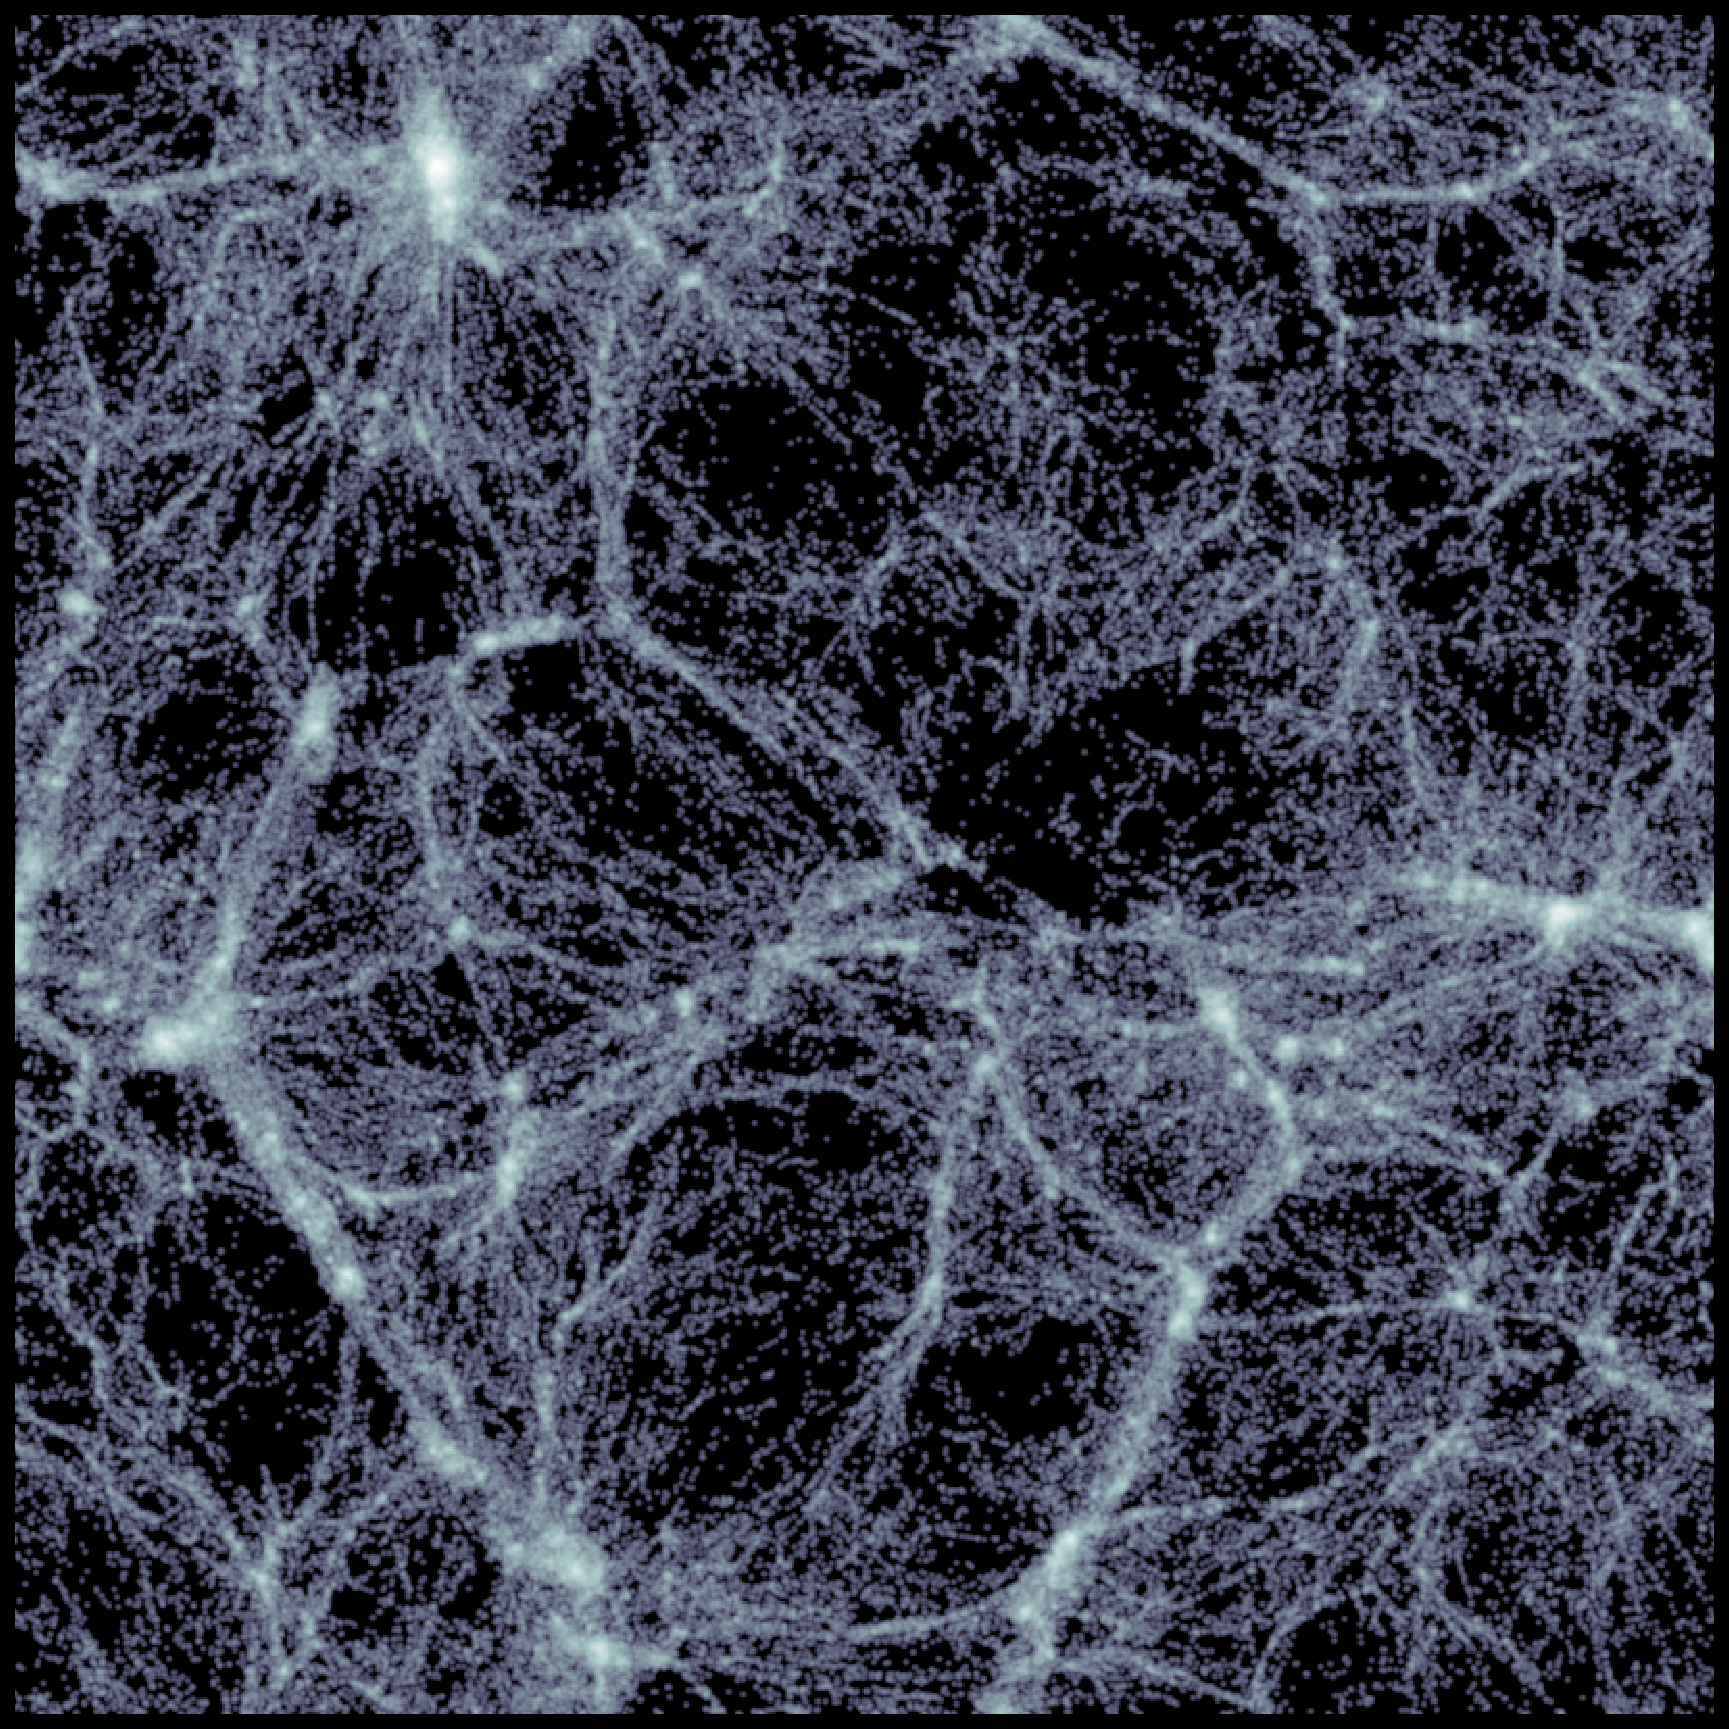
\includegraphics[width=\linewidth]{thesis/latex/intro_files/slice_image_bone.pdf}
    \caption{Distribution of galaxies in the IllustrisTNG100 simulation. Galaxies naturally trace the anisotropic nature of large scale structure formation, with large filamentary networks on multiple scales connecting the overdensities and encasing the underdensities. Colour scale goes from dark to light corresponding to low to high densities of galaxies.}
    \label{fig:cosmo_web_tng}
\end{figure}

As the baryonic gas flows within the gravitational potential well imposed by the web-like distribution of dark matter, material is advected giving rise to a fundamental connection between large scale structure and angular momentum in galaxies. Extending the formalism of TTT to include large scale structure formation \citep[e.g.][]{pichon2011,codis2015, laigle2015}, the angular momentum distribution of galaxies can be described relative to their neighbouring walls and filaments. In cosmological simulations, this can be seen as a mass dependent alignment between the spin of the dark matter haloes and the filament direction. The spin vectors of low mass haloes orient along the filament indicative of advection of angular momentum from the filament itself. Conversely high mass haloes have undergone mergers in the plane of the filament leading to a `flip' in orientation. How the spin of the haloes propogates to that of the baryonic components is complex and hence observations of this effect are inconclusive \citep[e.g.][]{tempel2013, krolewski2019, welker2020}. 

\section{Halo assembly bias}
As introduced in \S\ref{sec:ang_mom_intro}, bottom-up assembly in $\Lambda$CDM of dark matter haloes can be explained approximately by the excursion-set formalism which tracks the linear growth of primordial over-densities before spherically collapsing in the non-linear regime \citep{press1974,bond1991}. In the most basic form, environment is neglected and the assembly history of the halo is entirely dictated by its mass. This exclusive dependence on mass underlines the widely used halo occupation distribution \citep[HOD; e.g.][]{jing1998,peacock2000} modelling and various types of abundance matching \citep[e.g.][]{kravtsov2004,conroy2006}, which require galaxy clustering to be driven solely by halo mass \citep[e.g.][]{mo1996,sheth1999}. 

Parallel to the successes of HOD modelling, N-body simulations have fast converged on the fact that, at fixed halo mass, haloes which have formed at different times cluster differently \citep[e.g.][]{gao2005,wechsler2006,croton2007,wang2011}. Termed \textit{halo assembly bias}, this quantifies any physical quantity of a dark matter halo which correlates with halo clustering beyond the driving factor of halo mass. While most commonly considered as halo formation time, properties such as halo spin and concentration have also been demonstrated to be related with clustering \citep[e.g.][]{lacerna2012,lehmann2017}. 

Attempts to understand the origin of assembly bias have come from the large-scale tidal environment in which the given halo resides. Large-scale tidal forces are naturally anisotropic and intimately connected with the structure of the cosmic web. Halo assembly can therefore be de-convoluted as the influence of small and large scale forces. On small scales, gravity is dominant and the key properties are driven by local overdensity, encoded by the total mass of the halo. On large scales, the impact is more subtle \red{nuanced?}.

In simulations, \citet{hahn2009} found a systematic trend between halo formation time and the large-scale tidal force strength, derived from the geometric environment, at fixed halo mass. This effect is seen most strongly in low-mass haloes, arising from suppression of their growth when they reside within the vicinity of a much larger halo. This large halo acts to stop accretion on the low-mass halo in over-dense regions, effectively boosting the clustering of older low-mass haloes, compared to haloes of the same mass residing in under-dense regions that are less affected by tidal fields. \citet{ZOMGI} explore this phenomenon in the context of the cosmic web. Low-mass haloes residing within large filaments can often see their accretion `stalled' and hence will cease mass assembly earlier as matter flows preferentially along the filament to its densest points (nodes). Conversely low-mass haloes at the convergence point of multiple smaller filaments will have continued isotropic accretion resulting in longer continued mass growth and more recent formation. \citep[See][for a theoretical approach]{musso2018}.

Galaxies are our primary resource in probing the spatial distribution of dark matter. Their formation and subsequent evolution is tied to the assembly history of their host halo, however, determining the exact link is difficult. The observational counterpart of assembly bias is therefore tricky to isolate and as such is rightfully still under debate. In the context of galaxy evolution, the question of halo assembly bias can be rephrased to; \textit{does the cosmic web significantly impact galaxy evolution once stellar (or halo) mass has been accounted for?}

Early studies, however, have demonstrated observations of halo assembly bias. For example, \citet{tojeiro2017} compare a halo age proxy with respect to large-scale tidal environment defined in the Galaxy And Mass Assembly \citep[GAMA;][]{driver2009, driver2011} survey. They quantify tidal strength using the geometric classification of \citet{eardley2015} to characterise regions into geometric voids, sheets, filaments and knots corresponding to zero, one, two and three dimensions of collapse respectively. They find that low-mass haloes ($\lesssim 10^{12.5} M_{\odot}$) show a steadily increasing ratio of central galaxy stellar mass to total halo mass, corresponding to increasing halo age in regions of increasing tidal force strength (i.e. going from voids to knots). They find a tentative reversal of this trend for high-mass haloes ($\gtrsim 10^{13.2} M_{\odot}$). \citep[See][who explicitly look for changes in halo to stellar mass ratio with geometric environment using stacked lensing profiles, but find no significant changes when averaging over halo mass.]{brouwer2016}.

The tidal field can also be described in a topological sense with respect to the cosmic web. \citet{kraljic2018} provide an investigation in the GAMA survey through identification of the cosmic web, using the Discrete Persistent Structure Extractor code \citep[DisPerSE;][]{sousbie2011a,sousbie2011b}. \red{introduce disperse here?} They estimate distances to nodes, filaments and walls as a function of galaxy properties such as $u - r$ colour, specific star formation rate (sSFR) and stellar mass. They find distinct gradients with more massive, redder (passive) galaxies residing closer to nodes, filaments and walls, indicative of mass dependent clustering. Additionally, at fixed stellar mass, both star formation rate (SFR) decreases and colour reddens for galaxies closer to both nodes and filaments. Assuming the flow of baryonic accretion follows that of dark matter, this observation is consistent with the `stalling' of haloes due to tidal environment.

\section{This thesis}
In this thesis, I want to help answer three questions:

\begin{itemize}
    
    \item Why does the rotation of ionized gas decouple from the overall rotation of a galaxy, and how is this related to the angular momentum content of the dark matter halo?
    
    \item Are signatures of halo assembly bias detectable in galaxy observables such as kinematic misalignment or galaxy spin? \red{maybe rephrase this question?}
    
    \item How does the anisotropy of the cosmic web impact both the kinematics within galaxies and the dynamics of galaxies in the larger potential well of the overall halo?
    
\end{itemize}

In Chapter 2, I introduce the concept of kinematic misalignment and how this can be utilized in large scale Integral Field Spectroscopic surveys. In Chapter 3, I use an observational sample of misaligned galaxies to understand their typical characteristics and fundamental relationships with other observable properties. In Chapter 4, I introduce a mock observational sample created from a cosmological scale hydrodynamical simulation to understand if the observational trends can be reproduced and what can be learned from their evolutionary histories. In Chapter 5, I investigate the relationship between black hole activity in this mock sample and the relationship with kinematic misalignment. In Chapter 6, I investigate if kinematic misalignment in observations can be related to various measures of the assembly history of the surrounding dark matter halo. In Chapter 7, I investigate the differences between the orbits of satellite galaxies in different environments of the cosmic web and the potential for this to be recovered by dynamical models. In Chapter 8, I present results relating the spin alignment of galaxies with large scale structure in a large scale Integral Field Spectroscopic survey. In Chapter 9, I relate the angular momentum content of galaxies and dark matter haloes to the initial conditions of a hydrodynamical simulation.